\chapter{Discussion}
\label{chapter4}

%<Everything that comes under the `Results and Discussion' criterion in the mark scheme that has not been addressed in an earlier chapter should be included in this final chapter. The following section headings are suggestions only.>

\section{User Feedback and Analysis}

We will now discuss the results of user feedback and what they mean for the success of the project.

\subsection{Quantitative Results}

\begin{figure}[h]
\centering
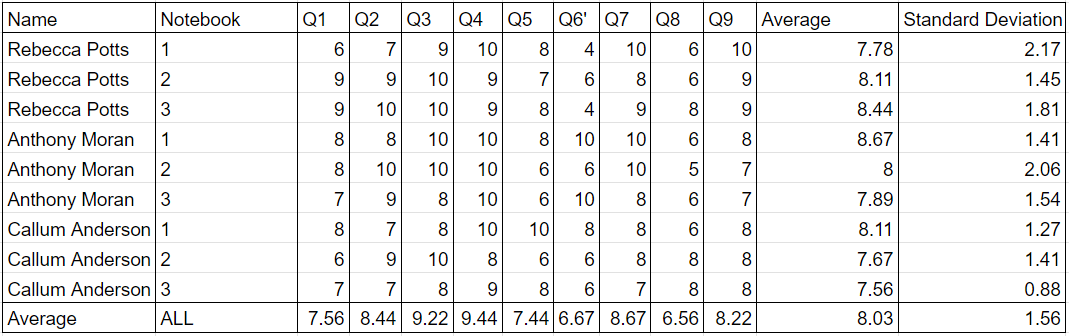
\includegraphics[width=\textwidth]{./images/misc/testing-results}
\caption{Quantitative results of user feedback}
\label{fig:user-feedback}
\end{figure}

The numerical results have been compiled into a table. Recall that Question 6 asked the user how difficult the notebooks were, with a more balanced result being more preferable. In hindsight, this was probably not a good idea. The question should have been phrased ``How balanced was the notebook?''. This is because in order to compute averages and perform other statistics correctly, all questions need to be on the same scale. Since the questionnaire has already been completed, the questions cannot be changed, so instead a transformation is applied to get the result in the same scale as the others. The closer to the middle, the higher the output. So 5 or 6 should be a 10, 5 or 7 should be an 8 and so on. The problem with this approach is that it increases the standard deviation of answers to this question, but it is the best we can do.

A few important statistics have been calculated in Figure \ref{fig:user-feedback}. Firstly, averages have been calculated for each submission along with the standard deviation. Then along the bottom row, averages have been calculated for each question and then finally the complete average and average standard deviation. This is a fairly crude metric of measuring success, since the sample size is quite small. Another problem with these statistics is that in order for the average score to equate with quality, we need to make the assumption that each question has equal impact on the quality of the notebook. This is just not true. It is hard to say what aspects are more important, and certain requirements might not even have a linear impact on the quality, for instance some might have diminishing returns.

However, if we do make that assumption, an average score of 8.03 quite good. The average standard deviation is 1.56, which is also acceptable. The lowest score presented is a 5 with all others being much higher than this. The lowest scoring question on average is Q8, asking how interesting the content was. The reason for such a low score here is probably due to sample size. This question is largely based on personal opinion and background. If one is not disposed to enjoying numerical methods and the mathematics involved, they may not find personal satisfaction in reading about a fairly complex method in that field. Based on the result it seems this cohort didn't have a particular love for the subject. The highest scoring question on average was Q4 which asked how prepared the readers were for the content presented to them. This is no surprise, all of the testers have a very similar background and the content was designed specifically to cater to this. It also means that content flowed well and the structure helped in preparing readers for upcoming content.

\subsection{Qualitative Results}

The testers were also encouraged to provide qualitative feedback through the form of comments boxes for each question. Some very useful feedback was provided, but it is too much to entirely cover here. However, some recurring points and potential problems will be highlighted.

Readability was overall rated well. Each tester had their own views, but largely it was said to be easy to read. One of their main concerns was with typos and grammatical mistakes. Another potential addition that sounded like a good idea was more underlining/emboldening of key terms, as this was already done to a small extent. For graphs and other visuals, the response was largely positive. All said they appreciated their inclusion and one said they ``made it easier to understand the content''. There were suggestions for more animated content and one tester found the curl diagrams a bit confusing.

Aesthetics had few comments, which makes sense since it is a very small part of what makes an effective notebook. This scored well and comments largely said that LaTeX looks very professional. There were a few comments about scroll bars appearing around long sections of text, which wasn't a problem on my system but I can understand how this might break up the flow of reading. Preparedness was good and its responses correlate with the fact it was the highest scoring question. One said that Notebook 3 ``built well on their knowledge of numerical methods''.

Usefulness is next and it seems some users expected to see more real-world application and motivations. The main user asking for this has a background in physics, which explains why their interest lies in the practical applications. Despite this potential bias, it is true that there could have been slightly more links to physical problems, since this is the motivation for studying FEM in the first place. Difficulty was an interesting one, it seemed by far that notebook 2 was the most difficult for people to digest, scoring 8 from all three testers. The other two notebooks were quite well balanced and people found them easier than hard. I think the perceived difficulty of notebook 2 can be explained by the density of mathematical material. Some said ``it became difficult to remember what [the symbols] meant'' and ``I thought it was pretty tough content''.

Structure was also rated quite well, tester said the material ``flowed naturally'' and was ``well broken down in the correct order''. The interest comments were another particularly personal one, as discussed before this did not score as well as the others and the comments reflect this. One tester said ``it's not boring or anything, its just pure maths'' for notebook 2. One even said ``for the most part I didn't understand a lot, which also affected my lack of interest''. This is unfortunate to hear, since the burden is on the author to make a subject accessible and easy to understand, not the student. However, with a larger sample size one would hope to see that students who have these kinds of experiences become the outliers. There were still positive comments, people seemed to find the gifs at the end of notebook 3 quite engaging. One said it ``made learning all the theory seem worth it''.

The final comments were instructive, people recommended that summaries be added to the end of the notebook, which seems like a good idea that was not thought of at the time. Some expressed an interest in more colour, more exercises and some specific changes, but overall the feedback was positive.

\section{Conclusions}

Overall, the project goals were met. The result is not fully polished, and could possibly be more extensive in its scope, but it succeeded in teaching students that the theory and implementation of the Finite Element Method is a fascinating subject. On the whole, testers walked away satisfied that they had learned something, even if they wouldn't personally use it for anything themselves.

With the notebooks designed in a scientific manner using Bloom's taxonomy and other sources to devise a criteria for successful learning resources, it can be said that the result is backed by existing research in the field of education.

\section{Ideas for future work} \label{section:ideas-for-future-work}

There are many ways this project could be expanded. Firstly, and most obviously, a more complete resource could be created. This would span many more types of PDE, including the Navier-Stokes fluid flow equations, Maxwell's electromagnetic equations, elastic deformation equations and more. Different solvers could be covered, other than LU Factorisation. Advanced meshing techniques like adaptive mesh refinement, complex valued functions, different types of finite element, a more in-depth look at function spaces. The list is endless because the field is so deep.

Other than expanding the syllabus, one could try using more modern technologies. Services like Brilliant and Khan Academy use sleek web design and videos to provide a more complete and smooth experience. Inspiration could be taken from them to build a web interface that hosts all the content. At the very least, getting Binder to work would help make the experience a bit smoother for students.